%==============================================================
%  EE201 -- Circuit Theory I
%  Lecture 17 : Capacitors
%  M. Mert Ankaralı, METU EEE
%
%  Compile:  ./build.sh      (or: pdflatex EE201_Lecture_17.tex, twice)
%==============================================================
\documentclass[11pt,a4paper]{article}

%-------------------- packages --------------------------------
\usepackage[T1]{fontenc}
\usepackage[utf8]{inputenc}
\usepackage[english]{babel}
\usepackage{lmodern}
\usepackage[left=2.2cm,right=4.4cm,top=2.2cm,bottom=2.2cm,headheight=14pt,headsep=9pt,marginparwidth=3.4cm,marginparsep=0.5cm]{geometry}
\usepackage{amsmath,amssymb}
\usepackage{array,booktabs,tabularx}
\usepackage{enumitem}
\usepackage{needspace}
\usepackage[table]{xcolor}
\usepackage{fancyhdr}
\usepackage{titlesec}
\usepackage{graphicx}
\usepackage[most]{tcolorbox}
\usepackage{tikz}
\usepackage[american,siunitx]{circuitikz}
\usetikzlibrary{matrix,arrows.meta,positioning,calc,decorations.pathmorphing,decorations.pathreplacing,decorations.markings,patterns,shapes.geometric}
\usepackage[colorlinks=true,allcolors=metured,breaklinks=true]{hyperref}

%-------------------- colour system ---------------------------
% One colour per physical quantity, used identically in the slides.
\definecolor{metured}{RGB}{155,27,48}    % headings, structure
\definecolor{metugray}{RGB}{88,89,91}
\definecolor{ccur}{RGB}{0,102,170}       % CURRENT  -- blue
\definecolor{cvolt}{RGB}{214,120,0}      % VOLTAGE  -- orange
\definecolor{cpow}{RGB}{23,128,74}       % POWER / ENERGY -- green
\definecolor{ccharge}{RGB}{124,60,160}   % CHARGE   -- purple
\definecolor{cflux}{RGB}{0,138,138}      % FLUX -- teal
\definecolor{boxgray}{RGB}{245,245,245}
\definecolor{copper}{RGB}{184,98,30}

\newcommand{\Icol}[1]{\textcolor{ccur}{#1}}
\newcommand{\Vcol}[1]{\textcolor{cvolt}{#1}}
\newcommand{\Pcol}[1]{\textcolor{cpow}{#1}}
\newcommand{\Qcol}[1]{\textcolor{ccharge}{#1}}
\newcommand{\Fcol}[1]{\textcolor{cflux}{#1}}

%-------------------- units (no siunitx dependency) -----------
\newcommand{\uni}[1]{\,\mathrm{#1}}
\newcommand{\A}{\uni{A}}   \newcommand{\V}{\uni{V}}
\newcommand{\W}{\uni{W}}   \newcommand{\J}{\uni{J}}
\newcommand{\Cb}{\uni{C}}  \newcommand{\s}{\uni{s}}
\newcommand{\Sie}{\uni{S}} \newcommand{\Wb}{\uni{Wb}}

%-------------------- layout ----------------------------------
\pagestyle{fancy}
\fancyhf{}
\lhead{\small\textcolor{metugray}{EE201 -- Circuit Theory I}}
\rhead{\small\textcolor{metugray}{Lecture 17: Capacitors}}
\cfoot{\small\thepage}
\renewcommand{\headrulewidth}{0.4pt}

\titleformat{\section}{\large\bfseries\color{metured}}{\thesection.}{0.6em}{}
\titleformat{\subsection}{\normalsize\bfseries\color{metugray}}{\thesubsection.}{0.6em}{}
\titlespacing*{\section}{0pt}{1.4ex plus .3ex}{0.7ex}
\titlespacing*{\subsection}{0pt}{1.1ex plus .2ex}{0.5ex}

\setlist[itemize]{itemsep=2pt,topsep=3pt,parsep=0pt,leftmargin=1.5em}
\setlist[enumerate]{itemsep=2pt,topsep=3pt,parsep=0pt,leftmargin=1.7em}
\setlength{\parindent}{0pt}
\setlength{\parskip}{1.2ex plus .2ex}
\linespread{1.25}
\AtBeginDocument{\setlength{\abovedisplayskip}{12pt plus 3pt}\setlength{\belowdisplayskip}{12pt plus 3pt}}
\raggedbottom
\widowpenalty=10000
\clubpenalty=10000
\brokenpenalty=10000

%-------------------- boxes -----------------------------------
\newtcolorbox{definitionbox}[1]{enhanced,
  colback=metured!4, colframe=metured, boxrule=0.9pt,
  fonttitle=\bfseries, title={#1}, arc=2pt,
  left=7pt,right=7pt,top=5pt,bottom=5pt, before skip=7pt, after skip=7pt,
  before upper={\setlength{\parskip}{0.6ex plus .1ex}}}

\newtcolorbox{ideabox}[1][Key idea]{enhanced,
  colback=ccur!5, colframe=ccur, boxrule=0.9pt,
  fonttitle=\bfseries, title={#1}, arc=2pt,
  left=7pt,right=7pt,top=5pt,bottom=5pt, before skip=7pt, after skip=7pt,
  before upper={\setlength{\parskip}{0.6ex plus .1ex}}}

\newtcolorbox{examplebox}[1][Example]{enhanced,
  colback=cpow!4, colframe=cpow, boxrule=0.9pt,
  fonttitle=\bfseries, title={#1}, arc=2pt,
  left=7pt,right=7pt,top=5pt,bottom=5pt, before skip=7pt, after skip=7pt,
  before upper={\setlength{\parskip}{0.6ex plus .1ex}}}

%  Example solutions: a heading and numbered steps outside the example box
\newif\ifsolfirst
\newcommand{\solution}{\par\smallskip\noindent{\color{cpow}\bfseries Solution}\par\nobreak\smallskip\global\solfirsttrue}
\newcommand{\solstep}[2]{\par\ifsolfirst\global\solfirstfalse\else\bigskip\fi
  \noindent{\color{cpow}\bfseries Step #1.}\ {\bfseries #2}\par\nobreak\smallskip}

\newtcolorbox{cautionbox}[1][Careful]{enhanced,
  colback=cvolt!6, colframe=cvolt, boxrule=0.9pt,
  fonttitle=\bfseries, title={#1}, arc=2pt,
  left=7pt,right=7pt,top=5pt,bottom=5pt, before skip=7pt, after skip=7pt,
  before upper={\setlength{\parskip}{0.6ex plus .1ex}}}

%-------------------- circuitikz defaults ---------------------
%  voltage sources: smaller + and - inside the circle, further apart
\ctikzset{bipoles/vsourceam/inner plus={\tiny$+$},
          bipoles/vsourceam/inner minus={\tiny$\vphantom{+}-$},
          bipoles/vsourceam/margin=0.85,
          bipoles/cvsourceam/inner plus={\tiny$+$},
          bipoles/cvsourceam/inner minus={\tiny$\vphantom{+}-$},
          bipoles/cvsourceam/margin=0.85}
\ctikzset{bipoles/length=0.9cm, color=black,
          label/align=straight,
          bipoles/generic/height=0.28, bipoles/generic/width=0.62}
\tikzset{
  iar/.style={-{Stealth[length=2.2mm]}, ccur, thick},
  pol/.style={font=\small, text=cvolt},
  glab/.style={font=\footnotesize, text=metured},
  ttl/.style={font=\scriptsize\bfseries, text=metugray},
  capn/.style={font=\scriptsize, text=metugray, align=center},
  bigarr/.style={-{Stealth[length=3mm]}, very thick, metugray},
  gnode/.style={circle, fill=metured, inner sep=0pt, minimum size=4.4pt},
  nlab/.style={circle, draw=metured, text=metured, font=\scriptsize, inner sep=0.7pt},
  blab/.style={font=\footnotesize, text=black!80},
  gbr/.style={black!75, thick, postaction={decorate, decoration={markings,
      mark=at position 0.56 with {\arrow{Stealth[length=2.5mm]}}}}},
  apbr/.style={ccur, line width=1.7pt, postaction={decorate, decoration={markings,
      mark=at position 0.56 with {\arrow{Stealth[length=2.8mm]}}}}},
  hal/.style={draw=cpow!60, line width=6pt, opacity=0.35, line cap=round, line join=round},
  elem/.style={draw=metugray, thick, fill=metulight},
}
\definecolor{metulight}{RGB}{243,240,241}

%-------------------- Lecture 17 macros: capacitors ---------------
\newcommand{\ohm}{\,\Omega}
\newcommand{\F}{\,\mathrm{F}}
\newcommand{\Jl}{\,\mathrm{J}}
\newcommand{\yes}{\textcolor{cpow}{\checkmark}}
\newcommand{\vC}{\Vcol{v_C}}
\newcommand{\iC}{\Icol{i_C}}
\newcommand{\iR}{\Icol{i_R}}
\newcommand{\Vo}{V_0}
\newcommand{\zm}{0^-}
\newcommand{\zp}{0^+}
\tikzset{vax/.style={-{Stealth[length=2mm]}, gray!70},
         crv/.style={metured, very thick, line join=round},
         crvu/.style={metured, very thick, dashed, line join=round},
         gdash/.style={black!45, densely dashed, thin},
         reg/.style={font=\scriptsize, text=metugray, align=center},
         imp/.style={metured, very thick, -{Stealth[length=2.6mm, width=2.4mm]}}}
%  axes and ticks in data units
\newcommand{\tax}[6]{\draw[vax] (#1,0) -- (#2,0) node[right, font=\small] {#5};
  \draw[vax] (0,#3) -- (0,#4) node[above, font=\small] {#6};}
\newcommand{\xt}[2]{\draw ([yshift=2pt]#1,0) -- ([yshift=-2pt]#1,0) node[below, font=\scriptsize] {#2};}
\newcommand{\xtu}[2]{\draw ([yshift=2pt]#1,0) -- ([yshift=-2pt]#1,0); \node[above, font=\scriptsize] at (#1,0) {#2};}
\newcommand{\yt}[2]{\draw ([xshift=2pt]0,#1) -- ([xshift=-2pt]0,#1) node[left, font=\scriptsize] {#2};}
\newcommand{\ytr}[2]{\draw ([xshift=2pt]0,#1) -- ([xshift=-2pt]0,#1); \node[right, font=\scriptsize] at (0,#1) {#2};}

%  ---------- singularity functions ----------
\newcommand{\stepPlot}{%
  \tax{-1.2}{2.4}{-0.3}{1.6}{$t$}{$u(t)$}
  \draw[crv] (-1.1,0) -- (0,0); \draw[crv] (0,1) -- (2.2,1); \yt{1}{$1$}}
\newcommand{\rampPlot}{%
  \tax{-1.2}{2.4}{-0.3}{1.9}{$t$}{$r(t)$}
  \draw[crv] (-1.1,0) -- (0,0) -- (1.7,1.7);
  \draw[gdash] (1,0) -- (1,1); \xt{1}{$1$}
  \node[font=\scriptsize, anchor=west] at (1.05,0.7) {slope $1$};}
\newcommand{\impPlot}{%
  \tax{-1.2}{2.4}{-0.3}{1.6}{$t$}{$\delta(t)$}
  \draw[crv] (-1.1,0) -- (2.2,0);
  \draw[imp] (0,0) -- (0,1.1); \node[font=\scriptsize, anchor=west] at (0.05,1.05) {$(1)$};}
\newcommand{\pulsePlot}{%
  \tax{-1.2}{2.4}{-0.3}{2.3}{$t$}{}
  \draw[crv] (-1.1,0) -- (0,0) -- (0,1.8) -- (0.6,1.8) -- (0.6,0) -- (2.2,0);
  \xt{0.6}{$\Delta$} \yt{1.8}{$1/\Delta$}
  \node[font=\scriptsize, anchor=west] at (0.7,1.5) {area $1$};}

%  ---------- the capacitor ----------
\newcommand{\capDef}{%
  \draw (0,2.2) node[ocirc] {} to[C, l=$C$, i>^=$\Icol{i}$] (0,0) node[ocirc] {};
  \node[pol] at (-0.55,1.85) {$+$}; \node[pol] at (-0.55,0.35) {$-$};
  \node[font=\small, text=cvolt] at (-0.6,1.1) {$v$};}
%  initial-condition models: #1 = 1, 2 or 3
\newcommand{\icModel}[1]{%
  \ifcase#1\or
    \draw (0,2.4) node[ocirc] {} to[C, l=$C$] (0,0) node[ocirc] {};
    \node[pol] at (-0.5,2.0) {$+$}; \node[pol] at (-0.5,0.4) {$-$};
    \node[font=\small, text=cvolt] at (-0.6,1.2) {$v$};
    \node[font=\scriptsize, align=center] at (0,-0.55) {$v(t_0^-) = \Vo$};
  \or
    \draw (0,2.4) node[ocirc] {} to[C, l=$C$] (0,1.2) to[american voltage source, l=$\Vo\,u(t - t_0)$] (0,-0.4) node[ocirc] {};
    \node[pol] at (-0.5,2.0) {$+$}; \node[pol] at (-0.5,0) {$-$};
    \node[font=\small, text=cvolt] at (-0.6,1.0) {$v$};
    \node[font=\scriptsize, align=center] at (0,-0.95) {uncharged};
  \or
    \draw (0,2.4) node[ocirc] {} -- (2.9,2.4); \draw (0,0) node[ocirc] {} -- (2.9,0);
    \draw (1.0,2.4) to[C, l=$C$] (1.0,0);
    \draw (2.9,0) to[american current source, l_=$C\Vo\,\delta(t - t_0)$] (2.9,2.4);
    \fill (1.0,0) circle (1.6pt); \fill (1.0,2.4) circle (1.6pt);
    \node[pol] at (-0.35,2.0) {$+$}; \node[pol] at (-0.35,0.4) {$-$};
    \node[font=\small, text=cvolt] at (-0.4,1.2) {$v$};
    \node[font=\scriptsize, align=center] at (1.4,-0.55) {uncharged};
  \fi}
%  parallel and series connections
\newcommand{\capPar}{%
  \draw (0,2) node[ocirc] {} -- (5.0,2); \draw (0,0) node[ocirc] {} -- (5.0,0);
  \draw (1.0,2) to[C, l=$C_1$] (1.0,0); \draw (2.4,2) to[C, l=$C_2$] (2.4,0);
  \node at (3.9,1) {$\cdots$}; \draw (5.0,2) to[C, l=$C_n$] (5.0,0);
  \fill (1.0,2) circle (1.6pt); \fill (2.4,2) circle (1.6pt); \fill (1.0,0) circle (1.6pt); \fill (2.4,0) circle (1.6pt);
  \node[pol] at (-0.3,1.7) {$+$}; \node[pol] at (-0.3,0.3) {$-$}; \node[font=\small, text=cvolt] at (-0.35,1) {$v$};}
\newcommand{\capSer}{%
  \draw (0,2) node[ocirc] {} to[C, l=$C_1$] (1.6,2) to[C, l=$C_2$] (3.2,2) -- (3.6,2);
  \node at (4.0,2) {$\cdots$};
  \draw (4.4,2) to[C, l=$C_n$] (5.8,2) -- (5.8,0) -- (0,0) node[ocirc] {};
  \node[pol] at (-0.3,1.7) {$+$}; \node[pol] at (-0.3,0.3) {$-$}; \node[font=\small, text=cvolt] at (-0.35,1) {$v$};}
%  current division: source i_s feeding C1 || C2
\newcommand{\cdiv}{%
  \draw (0,0) to[american current source, l=$\Icol{i_s}$] (0,2) -- (3.2,2);
  \draw (1.6,2) to[C, l=$C_1$, i>^=$\Icol{i_1}$] (1.6,0);
  \draw (3.2,2) to[C, l=$C_2$, i>^=$\Icol{i_2}$] (3.2,0) -- (0,0);
  \fill (1.6,2) circle (1.6pt); \fill (1.6,0) circle (1.6pt);}
%  voltage division: source, switch, C1 and C2 in series
\newcommand{\vdiv}{%
  \draw (0,0) to[american voltage source, l=$\Vcol{v_s}$, invert] (0,2.6) -- (1.8,2.6) to[cspst, l={$t = 0$}] (3.2,2.6) -- (3.2,2.5);
  \draw (3.2,2.5) to[C, l_=$C_1$] (3.2,1.3) to[C, l_=$C_2$] (3.2,0.1) -- (3.2,0) -- (0,0);
  \node[pol] at (3.75,2.3) {$+$}; \node[pol] at (3.75,1.5) {$-$}; \node[font=\small, text=cvolt] at (3.8,1.9) {$v_1$};
  \node[pol] at (3.75,1.1) {$+$}; \node[pol] at (3.75,0.3) {$-$}; \node[font=\small, text=cvolt] at (3.8,0.7) {$v_2$};}
%  parallel RC driven by a current source: #1 source label, #2 R, #3 C
\newcommand{\rcPar}[3]{%
  \draw (0,0) to[american current source, l=#1] (0,2.2) -- (3.6,2.2);
  \draw (1.8,2.2) to[R, l_=#2, i>^=$\iR$] (1.8,0);
  \draw (3.6,2.2) to[C, l=#3, i>^=$\iC$] (3.6,0) -- (0,0);
  \fill (1.8,2.2) circle (1.6pt); \fill (1.8,0) circle (1.6pt);
  \node[pol] at (2.75,1.85) {$+$}; \node[pol] at (2.75,0.35) {$-$}; \node[font=\small, text=cvolt] at (2.75,1.1) {$v_C$};}
%  capacitor discharged through a resistor at t = 0
\newcommand{\rcDis}{%
  \draw (0,0) to[C, l_=$C$] (0,2.2) -- (0.8,2.2) to[cspst, l={$t = 0$}] (2.2,2.2) -- (3.0,2.2) to[R, l=$R$, i>^=$\iR$] (3.0,0) -- (0,0);
  \node[pol] at (-0.5,1.85) {$+$}; \node[pol] at (-0.5,0.35) {$-$}; \node[font=\small, text=cvolt] at (-0.6,1.1) {$v_C$};}
%  two capacitors connected by a switch at t = 0
\newcommand{\twoCap}{%
  \draw (0,0) to[C, l_=$3\F$] (0,2.2) -- (0.8,2.2) to[cspst, l={$t = 0$}] (2.2,2.2) -- (3.0,2.2) to[C, l_=$6\F$] (3.0,0) -- (0,0);
  \node[pol] at (-0.5,1.85) {$+$}; \node[pol] at (-0.5,0.35) {$-$}; \node[font=\small, text=cvolt] at (-0.6,1.1) {$v_1$};
  \node[pol] at (3.55,1.85) {$+$}; \node[pol] at (3.55,0.35) {$-$}; \node[font=\small, text=cvolt] at (3.6,1.1) {$v_2$};}
\begin{document}

%-------------------- title block -----------------------------
\begin{center}
\begin{tcolorbox}[enhanced, colback=metured!5, colframe=metured, boxrule=1pt,
                  arc=3pt, left=10pt,right=10pt,top=7pt,bottom=7pt, width=\textwidth]
\begin{center}
  {\small\scshape Middle East Technical University}\\[2pt]
  {\small\scshape Department of Electrical and Electronics Engineering}\\[7pt]
  {\Large\bfseries\color{metured} EE201 -- Circuit Theory I}\\[4pt]
  {\large\bfseries Lecture 17: Capacitors}\\[6pt]
  {\small M. Mert Ankaral{\i}}
\end{center}
\end{tcolorbox}
\end{center}
\vspace{-0.5em}

\begin{center}
\small
\begin{tabular}{@{}l@{}}
\toprule
\textbf{Colour code used in these notes and in the slides}\\
\midrule
\Icol{$\blacksquare$}~current $i$ \quad
\Vcol{$\blacksquare$}~voltage $v$ \quad
\Pcol{$\blacksquare$}~energy $w$ \quad
\textcolor{metured}{$\blacksquare$}~waveform\\
\bottomrule
\end{tabular}
\end{center}

\textbf{Motivation.} Up to now every element was resistive: its voltage at time $t$ depends only
on its current at the same time $t$. Such circuits have no memory. A \textbf{capacitor} is
different. Its current depends on how fast its voltage changes, and it stores energy. Its
voltage now depends on the whole past of its current. This is the first \emph{dynamic} element
of the course. Circuits with capacitors are often switched on at some instant, so we first need
a few functions that describe sudden changes: the step, the ramp and the impulse.

%==============================================================
\section{Singularity functions}

\subsection{Step, ramp and impulse}

\begin{center}
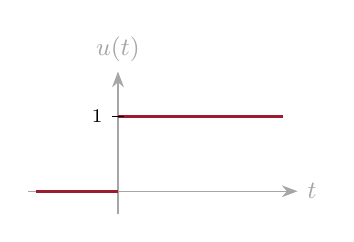
\begin{tikzpicture}[x=0.95cm,y=0.95cm]\stepPlot\end{tikzpicture}\hfill
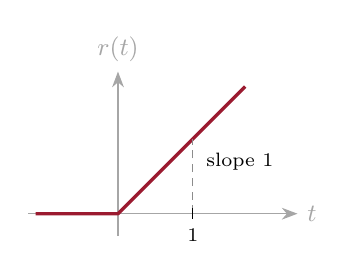
\begin{tikzpicture}[x=0.95cm,y=0.95cm]\rampPlot\end{tikzpicture}\hfill
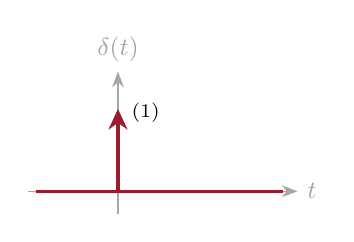
\begin{tikzpicture}[x=0.95cm,y=0.95cm]\impPlot\end{tikzpicture}
\end{center}

\[
  u(t) = \begin{cases} 1, & t > 0\\ 0, & t < 0 \end{cases}
  \qquad
  r(t) = \begin{cases} t, & t \geq 0\\ 0, & t < 0 \end{cases}
\]
The \textbf{unit step} $u(t)$ switches on at $t = 0$. The \textbf{unit ramp} $r(t)$ grows with
slope $1$ from $t = 0$. The \textbf{unit impulse} $\delta(t)$ needs more care.

\subsection{The unit impulse}

\begin{minipage}[c]{0.42\linewidth}
\centering
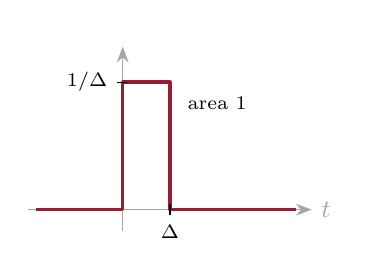
\begin{tikzpicture}[x=1.0cm,y=0.9cm]\pulsePlot\end{tikzpicture}
\end{minipage}\hfill
\begin{minipage}[c]{0.54\linewidth}
Take a pulse of width $\Delta$ and height $1/\Delta$:
\[
  \frac{u(t) - u(t - \Delta)}{\Delta} .
\]
Its area is $1$ for every $\Delta$. Let $\Delta \to 0$: the pulse gets narrower and taller, but
its area stays $1$.
\end{minipage}

\begin{definitionbox}{Unit impulse}
\[
  \delta(t) = \lim_{\Delta \to 0} \frac{u(t) - u(t - \Delta)}{\Delta}
\]
\[
  \delta(t) = 0 \ \text{for } t \neq 0,
  \qquad
  \int_{-\alpha}^{\beta} \delta(t)\,dt = 1 \ \text{for all } \alpha, \beta > 0 .
\]
\end{definitionbox}

At $t = 0$ the impulse is not a number; it is \emph{singular}. Only its area means something. In
drawings it is an arrow, with its area written in brackets.

The three functions are linked by integration and differentiation:
\[
  \int_{-\infty}^{t} \delta(\tau)\,d\tau = u(t),
  \qquad
  \int_{-\infty}^{t} u(\tau)\,d\tau = r(t),
  \qquad
  \frac{d}{dt}\,r(t) = u(t),
  \qquad
  \frac{d}{dt}\,u(t) = \delta(t) .
\]
The last one is a convention: a jump of size $1$ has an impulse of area $1$ as its derivative.
More generally, a jump of size $a$ at $t_0$ gives $a\,\delta(t - t_0)$ in the derivative.

\begin{examplebox}[Example 17.1 --- from a formula to a sketch]
Sketch $f(t) = 2\,u(-t - 1)$.
\end{examplebox}

\solution

\begin{minipage}[c]{0.56\linewidth}
Let $s = -t - 1$. Then $2u(s) = 2$ for $s > 0$, that is for $t < -1$, and $0$ for $t > -1$:
\[
  f(t) = \begin{cases} 2, & t < -1\\ 0, & t > -1 . \end{cases}
\]
The minus sign in front of $t$ flips the step: it is on for $t$ to the \emph{left} of $-1$.
\end{minipage}\hfill
\begin{minipage}[c]{0.4\linewidth}
\centering
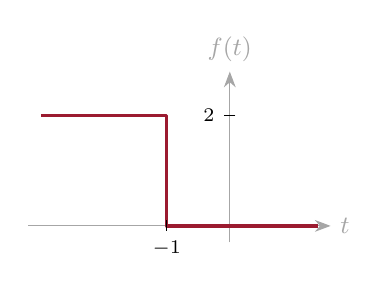
\begin{tikzpicture}[x=0.8cm,y=0.7cm]
  \tax{-3.2}{1.6}{-0.3}{2.8}{$t$}{$f(t)$}
  \draw[crv] (-3.0,2) -- (-1,2) -- (-1,0) -- (1.4,0);
  \xt{-1}{$-1$} \yt{2}{$2$}
\end{tikzpicture}
\end{minipage}

\begin{examplebox}[Example 17.2 --- from a sketch to a formula]
\begin{minipage}[c]{0.4\linewidth}
\centering
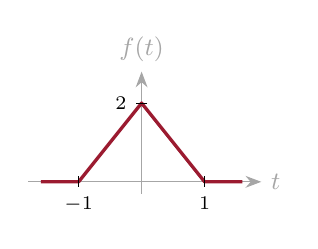
\begin{tikzpicture}[x=0.8cm,y=0.5cm]
  \tax{-1.8}{1.9}{-0.3}{2.8}{$t$}{$f(t)$}
  \draw[crv] (-1.6,0) -- (-1,0) -- (0,2) -- (1,0) -- (1.6,0);
  \xt{-1}{$-1$} \xt{1}{$1$} \yt{2}{$2$}
\end{tikzpicture}
\end{minipage}\hfill
\begin{minipage}[c]{0.56\linewidth}
Write the triangle $f(t)$ in terms of ramps.
\end{minipage}
\end{examplebox}

\solution

Build the slope from left to right. At $t = -1$ the slope becomes $+2$: add $2r(t + 1)$. At
$t = 0$ the slope must become $-2$, a change of $-4$: add $-4r(t)$. At $t = 1$ it must become
$0$, a change of $+2$: add $2r(t - 1)$.
\[
  f(t) = 2\,r(t + 1) - 4\,r(t) + 2\,r(t - 1) .
\]
\begin{center}
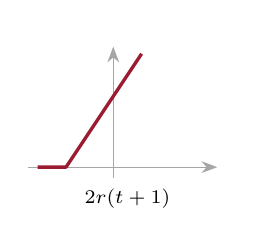
\begin{tikzpicture}[x=0.6cm,y=0.45cm]
  \tax{-1.8}{2.2}{-0.3}{3.4}{}{}
  \draw[crv] (-1.6,0) -- (-1,0) -- (0.6,3.2); \node[font=\scriptsize] at (0.3,-0.9) {$2r(t+1)$};
\end{tikzpicture}\quad
\raisebox{0.6cm}{$+$}\quad
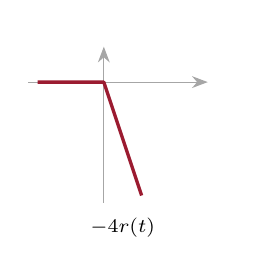
\begin{tikzpicture}[x=0.6cm,y=0.45cm]
  \tax{-1.6}{2.2}{-3.4}{1.0}{}{}
  \draw[crv] (-1.4,0) -- (0,0) -- (0.8,-3.2); \node[font=\scriptsize] at (0.4,-4.1) {$-4r(t)$};
\end{tikzpicture}\quad
\raisebox{0.6cm}{$+$}\quad
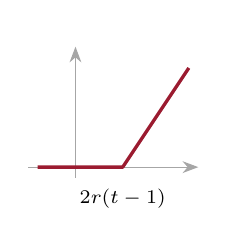
\begin{tikzpicture}[x=0.6cm,y=0.45cm]
  \tax{-1.0}{2.6}{-0.3}{3.4}{}{}
  \draw[crv] (-0.8,0) -- (1,0) -- (2.4,2.8); \node[font=\scriptsize] at (1.0,-0.9) {$2r(t-1)$};
\end{tikzpicture}
\end{center}

\begin{examplebox}[Example 17.3 --- derivatives give impulses]
\begin{minipage}[c]{0.44\linewidth}
\centering
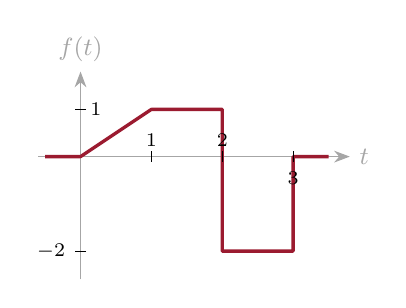
\begin{tikzpicture}[x=0.9cm,y=0.6cm]
  \tax{-0.6}{3.8}{-2.6}{1.8}{$t$}{$f(t)$}
  \draw[crv] (-0.5,0) -- (0,0) -- (1,1) -- (2,1) -- (2,-2) -- (3,-2) -- (3,0) -- (3.5,0);
  \xtu{1}{$1$} \xtu{2}{$2$} \xt{3}{$3$} \ytr{1}{$1$} \yt{-2}{$-2$}
\end{tikzpicture}
\end{minipage}\hfill
\begin{minipage}[c]{0.52\linewidth}
Write $f(t)$ with ramps and steps, and find $\dot f(t) = df/dt$.
\end{minipage}
\end{examplebox}

\solution

\solstep{1}{The function}
A ramp starts at $t = 0$ and stops at $t = 1$; at $t = 2$ the function jumps by $-3$; at $t = 3$
it jumps by $+2$:
\[
  f(t) = r(t) - r(t - 1) - 3\,u(t - 2) + 2\,u(t - 3) .
\]

\solstep{2}{The derivative}
Differentiate term by term ($\dot r = u$, $\dot u = \delta$):

\begin{minipage}[c]{0.52\linewidth}
\[
  \dot f(t) = u(t) - u(t - 1) - 3\,\delta(t - 2) + 2\,\delta(t - 3) .
\]
Each jump of $f$ gives an impulse in $\dot f$ whose area is the size of the jump.
\end{minipage}\hfill
\begin{minipage}[c]{0.44\linewidth}
\centering
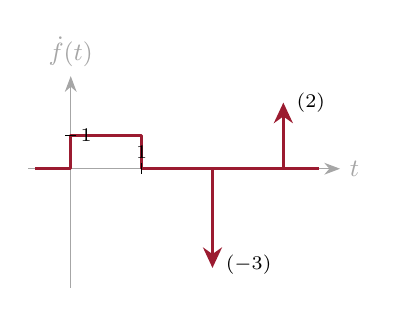
\begin{tikzpicture}[x=0.9cm,y=0.42cm]
  \tax{-0.6}{3.8}{-3.6}{2.8}{$t$}{$\dot f(t)$}
  \draw[crv] (-0.5,0) -- (0,0) -- (0,1) -- (1,1) -- (1,0) -- (3.5,0);
  \draw[imp] (2,0) -- (2,-3); \node[font=\scriptsize, anchor=west] at (2.05,-2.9) {$(-3)$};
  \draw[imp] (3,0) -- (3,2); \node[font=\scriptsize, anchor=west] at (3.05,2.0) {$(2)$};
  \xtu{1}{$1$} \ytr{1}{$1$}
\end{tikzpicture}
\end{minipage}

\subsection{The sifting property}

Multiply a continuous function $f(t)$ by $\delta(t)$. Since $\delta(t) = 0$ for $t \neq 0$, only
the value $f(0)$ matters:
\[
  \int_{-T}^{T} f(t)\,\delta(t)\,dt = f(0) \qquad (T > 0).
\]
To see this, use the pulse: $\displaystyle \int f(t)\,\frac{u(t) - u(t - \Delta)}{\Delta}\,dt
= \frac{1}{\Delta}\int_0^{\Delta} f(t)\,dt$, the average of $f$ over $[0, \Delta]$, which tends
to $f(0)$ as $\Delta \to 0$. Shifted to $t_0$:
\[
  \boxed{\ f(t)\,\delta(t - t_0) = f(t_0)\,\delta(t - t_0) \ }
  \qquad (f \text{ continuous at } t_0).
\]
The impulse ``sifts out'' the value of $f$ at $t_0$.

%==============================================================
\section{The linear time-invariant capacitor}

\begin{minipage}[c]{0.3\linewidth}
\centering
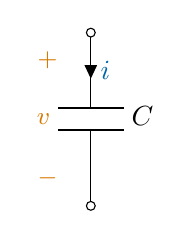
\begin{tikzpicture}[scale=1.0]\capDef\end{tikzpicture}
\end{minipage}\hfill
\begin{minipage}[c]{0.66\linewidth}
A capacitor stores charge $q$ in proportion to its voltage, and its current is the rate of change
of the charge:
\[
  q(t) = C\,\Vcol{v(t)}, \qquad \Icol{i(t)} = \frac{dq}{dt} .
\]
$C$ is the \textbf{capacitance}, measured in farads (F). The reference directions follow the
passive convention.
\end{minipage}

\begin{definitionbox}{LTI capacitor}
\[
  \Icol{i(t)} = C\,\frac{d\Vcol{v(t)}}{dt}
  \qquad\Longleftrightarrow\qquad
  \Vcol{v(t)} = \Vcol{v(t_0)} + \frac{1}{C}\int_{t_0}^{t} \Icol{i(\tau)}\,d\tau .
\]
\end{definitionbox}

Two consequences follow directly.
\begin{itemize}
  \item If $v$ is constant (DC), then $i = 0$: in DC steady state a capacitor is an \textbf{open
        circuit}.
  \item The voltage now depends on the initial voltage $v(t_0)$ \emph{and} on the whole current
        between $t_0$ and $t$: the capacitor has \textbf{memory}.
\end{itemize}

\subsection{Energy}

The power delivered to the capacitor is $p(t) = v(t)\,i(t)$. The energy delivered during
$[t_0, t]$ is
\[
  \Pcol{w(t_0, t)} = \int_{t_0}^{t} v\,i\,d\tau = \int_{t_0}^{t} v\,C\,\frac{dv}{d\tau}\,d\tau
  = \int_{v(t_0)}^{v(t)} C\,v\,dv = \tfrac12 C\,v(t)^2 - \tfrac12 C\,v(t_0)^2 .
\]
Take $t_0 \to -\infty$ and assume the capacitor was uncharged long ago ($v(-\infty) = 0$). The
energy \textbf{stored} at time $t$ is
\[
  \boxed{\ \Pcol{w(t)} = \tfrac12\,C\,\Vcol{v(t)}^2 \ }
\]
It depends only on the present voltage. It is never negative, so the capacitor never delivers
more energy than it received: it is a \emph{passive} element. Delivered energy is not lost; it is
stored, and can be given back.

\begin{examplebox}[Example 17.4 --- current and energy from a voltage waveform]
A $2\F$ capacitor has $\Vcol{v(t)} = r(t) - r(t - 1)$ V. Find $\Icol{i(t)}$ and the stored energy
for $t \geq 1$. What would the current be if instead $\Vcol{v(t)} = u(t)$ V?
\end{examplebox}

\solution

\begin{minipage}[c]{0.52\linewidth}
\solstep{1}{Current}
$v$ rises from $0$ to $1\V$ during $[0, 1]$ and then stays at $1\V$:
\[
  \Icol{i(t)} = 2\,\frac{d}{dt}\big[r(t) - r(t - 1)\big]
\]
\[
  \Icol{i(t)} = 2\,\big[u(t) - u(t - 1)\big] \ \mathrm{A}.
\]
\solstep{2}{Energy}
For $t \geq 1$: $\ \Pcol{w} = \tfrac12 \cdot 2 \cdot 1^2 = 1\Jl$, and no current flows.
\end{minipage}\hfill
\begin{minipage}[c]{0.44\linewidth}
\centering
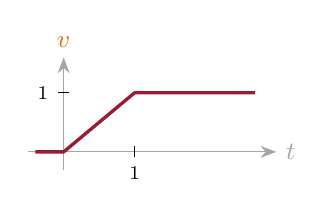
\begin{tikzpicture}[x=0.9cm,y=0.75cm]
  \tax{-0.5}{3.0}{-0.3}{1.6}{$t$}{$\Vcol{v}$}
  \draw[crv] (-0.4,0) -- (0,0) -- (1,1) -- (2.7,1); \xt{1}{$1$} \yt{1}{$1$}
\end{tikzpicture}\\[4pt]
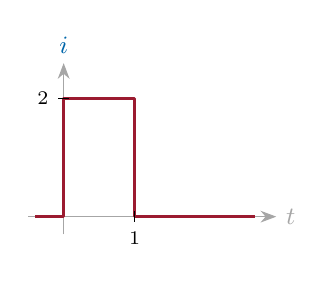
\begin{tikzpicture}[x=0.9cm,y=0.75cm]
  \tax{-0.5}{3.0}{-0.3}{2.6}{$t$}{$\Icol{i}$}
  \draw[crv] (-0.4,0) -- (0,0) -- (0,2) -- (1,2) -- (1,0) -- (2.7,0); \xt{1}{$1$} \yt{2}{$2$}
\end{tikzpicture}
\end{minipage}

\solstep{3}{A jump in voltage}
If $\Vcol{v(t)} = u(t)$ V, then $\Icol{i(t)} = 2\,\delta(t)$ A. A sudden jump in capacitor
voltage needs an \emph{impulse} of current. With bounded currents, the capacitor voltage cannot
jump.

%==============================================================
\section{Initial-condition models}

A capacitor charged to $\Vo$ at $t_0$ can be replaced, for $t > t_0$, by an \emph{uncharged}
capacitor and a source. Three equivalent models:

\begin{center}
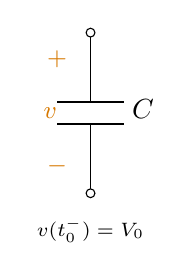
\begin{tikzpicture}[scale=0.85]\icModel{1}\end{tikzpicture}
\hspace{0.6cm}\raisebox{1cm}{$\equiv$}\hspace{0.6cm}
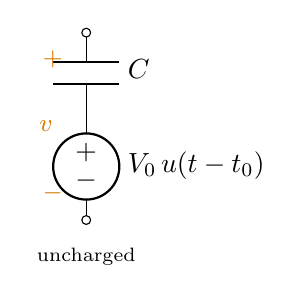
\begin{tikzpicture}[scale=0.85]\icModel{2}\end{tikzpicture}
\hspace{0.9cm}\raisebox{1cm}{$\equiv$}\hspace{0.4cm}
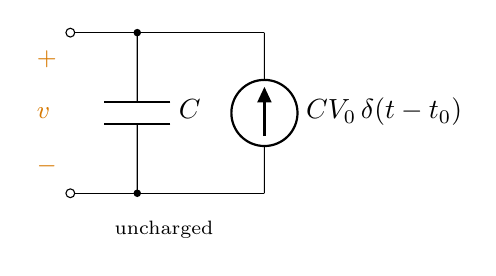
\begin{tikzpicture}[scale=0.85]\icModel{3}\end{tikzpicture}
\end{center}
\begin{center}
\small
\begin{tabular}{@{}lll@{}}
model 1 & model 2 & model 3\\
charged, $v(t_0^-) = \Vo$ & uncharged $C$ $+$ voltage step & uncharged $C$ $\parallel$ current impulse
\end{tabular}
\end{center}

``Equivalent'' means: for $t > t_0$ all three give the same $v(t)$ for the same $i(t)$ at the
terminals.

\textbf{Model 1.} $\ v(t) = v(t_0^-) + \frac1C\int_{t_0^-}^{t} i\,d\tau = \Vo + \frac1C\int_{t_0^-}^{t} i\,d\tau$.

\textbf{Model 2.} The capacitor starts at $0$; the source adds $\Vo\,u(t - t_0) = \Vo$ for
$t > t_0$:
\[
  v(t) = 0 + \frac1C\int_{t_0^-}^{t} i\,d\tau + \Vo .
\]

\textbf{Model 3.} The capacitor current is $i(\tau) + C\Vo\,\delta(\tau - t_0)$:
\[
  v(t) = 0 + \frac1C\int_{t_0^-}^{t} \big[i(\tau) + C\Vo\,\delta(\tau - t_0)\big]\,d\tau
  = \Vo + \frac1C\int_{t_0^-}^{t} i\,d\tau .
\]
All three agree. Model 2 is handy in series connections, model 3 in parallel connections. The
impulse in model 3 is exactly the charge $C\Vo$ delivered in an instant.

%==============================================================
\section{Connections and division}

\subsection{Parallel capacitors}

\begin{minipage}[c]{0.44\linewidth}
\centering
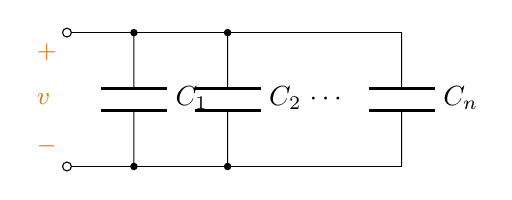
\begin{tikzpicture}[scale=0.85]\capPar\end{tikzpicture}
\end{minipage}\hfill
\begin{minipage}[c]{0.52\linewidth}
All capacitors have the same voltage $v$, with $v(t_0) = \Vo$. KCL:
\[
  i = C_1\frac{dv}{dt} + \cdots + C_n\frac{dv}{dt} = (C_1 + \cdots + C_n)\frac{dv}{dt} .
\]
\end{minipage}
\[
  \boxed{\ C_{eq} = C_1 + C_2 + \cdots + C_n \ }, \qquad v_{eq}(t_0) = \Vo .
\]
Capacitors in parallel add like conductances.

\subsection{Series capacitors}

\begin{minipage}[c]{0.5\linewidth}
\centering
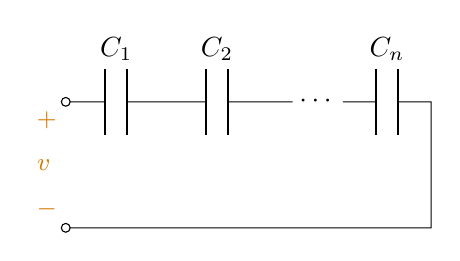
\begin{tikzpicture}[scale=0.8]\capSer\end{tikzpicture}
\end{minipage}\hfill
\begin{minipage}[c]{0.46\linewidth}
All capacitors carry the same current $i$. Capacitor $k$ starts at $v_k(t_0) = V_{k0}$. KVL:
$v = v_1 + \cdots + v_n$.
\end{minipage}
\[
  v(t) = \sum_k \Big( V_{k0} + \frac{1}{C_k}\int_{t_0}^{t} i\,d\tau \Big)
  = \underbrace{\big(V_{10} + \cdots + V_{n0}\big)}_{v(t_0)}
  + \underbrace{\Big(\frac{1}{C_1} + \cdots + \frac{1}{C_n}\Big)}_{1/C_{eq}} \int_{t_0}^{t} i\,d\tau .
\]
\[
  \boxed{\ \frac{1}{C_{eq}} = \frac{1}{C_1} + \frac{1}{C_2} + \cdots + \frac{1}{C_n} \ },
  \qquad v_{eq}(t_0) = V_{10} + \cdots + V_{n0} .
\]
Capacitors in series combine like resistors in parallel; their initial voltages add.

\subsection{Current division}

\begin{minipage}[c]{0.4\linewidth}
\centering
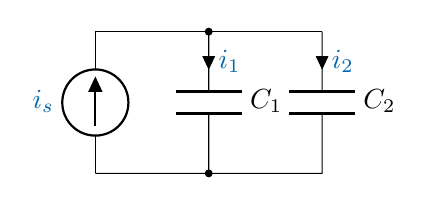
\begin{tikzpicture}[scale=0.9]\cdiv\end{tikzpicture}
\end{minipage}\hfill
\begin{minipage}[c]{0.56\linewidth}
Same voltage: $\ \frac{dv}{dt} = \frac{\Icol{i_1}}{C_1} = \frac{\Icol{i_2}}{C_2}$.
KCL: $\ \Icol{i_1} + \Icol{i_2} = \Icol{i_s}$. Hence
\[
  \Icol{i_1} = \frac{C_1}{C_1 + C_2}\,\Icol{i_s},
  \qquad
  \Icol{i_2} = \frac{C_2}{C_1 + C_2}\,\Icol{i_s} .
\]
The larger capacitor takes the larger share.
\end{minipage}

\subsection{Voltage division}

\begin{minipage}[c]{0.4\linewidth}
\centering
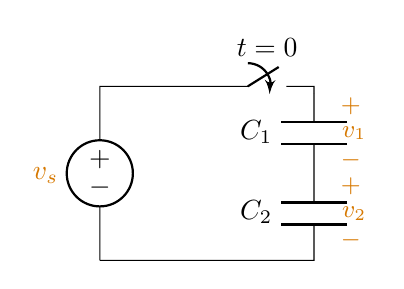
\begin{tikzpicture}[scale=0.85]\vdiv\end{tikzpicture}
\end{minipage}\hfill
\begin{minipage}[c]{0.56\linewidth}
Before the switch closes, $v_1(0^-) = V_{10}$ and $v_2(0^-) = V_{20}$. For $t > 0$ the same
current flows in both:
\[
  \int_{0^-}^{t} i\,d\tau = C_1\big(v_1 - V_{10}\big) = C_2\big(v_2 - V_{20}\big) .
\]
KVL: $v_1 + v_2 = v_s$.
\end{minipage}
\begin{align*}
  \Vcol{v_1(t)} &= \frac{C_2}{C_1 + C_2}\,\Vcol{v_s(t)} + \frac{C_1 V_{10} - C_2 V_{20}}{C_1 + C_2}\\
  \Vcol{v_2(t)} &= \frac{C_1}{C_1 + C_2}\,\Vcol{v_s(t)} + \frac{C_2 V_{20} - C_1 V_{10}}{C_1 + C_2}
  \qquad (t > 0).
\end{align*}
For example, $C_1 = 1\F$, $C_2 = 2\F$, $v_s = 6\V$ and both uncharged: $v_1 = 4\V$, $v_2 = 2\V$.
The \emph{smaller} capacitor takes the larger voltage. If instead $V_{10} = 3\V$:
$v_1 = (12 + 3)/3 = 5\V$ and $v_2 = 1\V$.

%==============================================================
\section{From $t = 0^-$ to $t = 0^+$}

When a source switches on or a switch closes at $t = 0$, we need the values just after, at
$t = 0^+$, from the values just before, at $t = 0^-$.

\begin{ideabox}[Finite energy and the capacitor voltage]
We assume that the energy stored in a capacitor is always finite. Since $w = \frac12 C v_C^2$,
the capacitor voltage $v_C$ is always \textbf{bounded}. Then:
\begin{itemize}
  \item If the capacitor current $i_C$ is bounded on $[0^-, 0^+]$, then
        $\ v_C(0^+) = v_C(0^-) + \frac1C\int_{0^-}^{0^+} i_C\,d\tau = v_C(0^-)$:
        \textbf{the capacitor voltage is continuous}.
  \item Only an \emph{impulse} of current can make $v_C$ jump.
\end{itemize}
To find what happens during $0^- < t < 0^+$, replace the capacitor by a bounded voltage source
$v_C(t)$ (substitution theorem) and check which currents stay bounded.
\end{ideabox}

\begin{examplebox}[Example 17.5 --- a step source]
\begin{minipage}[c]{0.48\linewidth}
\centering
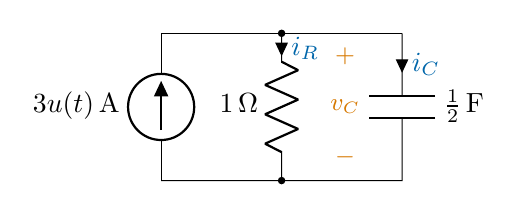
\begin{tikzpicture}[scale=0.85]\rcPar{$3u(t)\,\mathrm{A}$}{$1\ohm$}{$\tfrac12\F$}\end{tikzpicture}
\end{minipage}\hfill
\begin{minipage}[c]{0.48\linewidth}
Find $\vC(0^+)$, $\iR(0^+)$ and $\iC(0^+)$ when\\
(a) $\vC(0^-) = 0$, \quad (b) $\vC(0^-) = 4\V$.
\end{minipage}
\end{examplebox}

\solution

\solstep{1}{During $0^- < t < 0^+$}
Replace the capacitor by a voltage source $\vC(t)$. It is bounded (finite energy), so
$\iR = \vC / 1$ is bounded. KCL: $\iC = 3u(t) - \iR$, a bounded current. Hence
\[
  \vC(0^+) = \vC(0^-) + 2\int_{0^-}^{0^+} \iC\,d\tau = \vC(0^-) .
\]

\solstep{2}{At $t = 0^+$}
The source gives $3\,\mathrm{A}$, the capacitor holds its voltage:
\begin{center}
\renewcommand{\arraystretch}{1.3}
\begin{tabular}{@{}lccc@{}}
\toprule
& $\vC(0^+)$ & $\iR(0^+) = \vC(0^+)/1$ & $\iC(0^+) = 3 - \iR(0^+)$\\
\midrule
(a) $\vC(0^-) = 0$ & $0$ & $0$ & $3\,\mathrm{A}$\\
(b) $\vC(0^-) = 4\V$ & $4\V$ & $4\,\mathrm{A}$ & $-1\,\mathrm{A}$\\
\bottomrule
\end{tabular}
\end{center}
At the switching instant the capacitor behaves like a voltage source equal to its initial
voltage (a short circuit if uncharged). The currents may jump; the capacitor voltage does not.

\begin{examplebox}[Example 17.6 --- an impulse source]
\begin{minipage}[c]{0.48\linewidth}
\centering
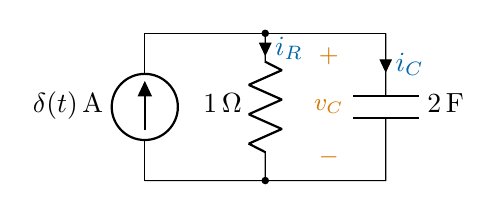
\begin{tikzpicture}[scale=0.85]\rcPar{$\delta(t)\,\mathrm{A}$}{$1\ohm$}{$2\F$}\end{tikzpicture}
\end{minipage}\hfill
\begin{minipage}[c]{0.48\linewidth}
$\vC(0^-) = 1\V$. Find $\vC(0^+)$, $\iR(0^+)$ and $\iC(0^+)$.
\end{minipage}
\end{examplebox}

\solution

\solstep{1}{During $0^- < t < 0^+$}
$\vC$ is bounded, so $\iR = \vC/1$ is bounded. KCL: $\iC = \delta(t) - \iR$. Now
\begin{align*}
  \vC(0^+) &= \vC(0^-) + \frac12\int_{0^-}^{0^+} \big[\delta(\tau) - \iR(\tau)\big]\,d\tau\\
  &= 1 + \frac12 \cdot 1 - \underbrace{\frac12\int_{0^-}^{0^+} \iR\,d\tau}_{0}
  = 1.5\V .
\end{align*}
The impulse of current goes entirely into the capacitor and charges it by
$1/C = 0.5\V$ in an instant.

\solstep{2}{At $t = 0^+$}
The source is zero again: $\iR(0^+) = 1.5\,\mathrm{A}$ and $\iC(0^+) = -\iR(0^+) = -1.5\,\mathrm{A}$.

\begin{cautionbox}[Where does the impulse go?]
During $0^- < t < 0^+$ we found $\iC = \delta(t) - \iR$: an impulsive part plus a bounded part.
The bounded part has no effect on $\vC(0^+)$. So, to find the impulsive part, we may replace the
capacitor by \emph{any} bounded voltage source, in particular by a \textbf{short circuit}. Then
the impulse of current clearly flows through the short (the capacitor), not through the
resistor.
\end{cautionbox}

%==============================================================
\section{Energy examples}

\begin{examplebox}[Example 17.7 --- an RC circuit discharging]
\begin{minipage}[c]{0.44\linewidth}
\centering
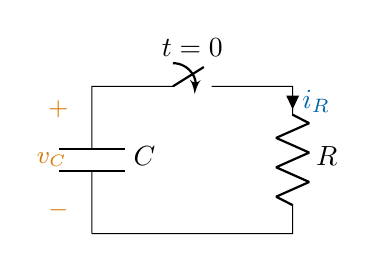
\begin{tikzpicture}[scale=0.85]\rcDis\end{tikzpicture}
\end{minipage}\hfill
\begin{minipage}[c]{0.52\linewidth}
$\vC(0^-) = \Vo$. The switch closes at $t = 0$. Find $\vC(t)$ and $\iR(t)$ for $t > 0$, and follow
the energy.
\end{minipage}
\end{examplebox}

\solution

\solstep{1}{Initial value}
The current through the resistor is bounded ($\iR = \vC / R$, $\vC$ bounded), so
$\vC(0^+) = \vC(0^-) = \Vo$.

\solstep{2}{For $t > 0$}
The capacitor current is $\iC = -\iR$ (same loop, opposite reference) and $\vC = R\,\iR$:
\[
  C\,\frac{d\vC}{dt} = -\frac{\vC}{R}
  \quad\Rightarrow\quad
  \frac{d\vC}{dt} = -\frac{1}{RC}\,\vC
\]
\[
  \vC(t) = \Vo\,e^{-t/RC}, \qquad \iR(t) = \frac{\Vo}{R}\,e^{-t/RC} \qquad (t > 0).
\]
(Check: $\frac{d}{dt}\Vo e^{-t/RC} = -\frac{1}{RC}\Vo e^{-t/RC}$, and the value at $0^+$ is
$\Vo$.)

\begin{center}
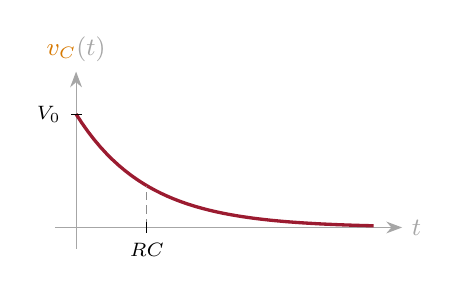
\begin{tikzpicture}[x=0.9cm,y=0.9cm]
  \tax{-0.3}{4.6}{-0.3}{2.2}{$t$}{$\vC(t)$}
  \draw[crv, domain=0:4.2, samples=50] plot (\x, {1.6*exp(-\x)});
  \yt{1.6}{$\Vo$}
  \draw[gdash] (1,0) -- (1,{1.6*exp(-1)}); \xt{1}{$RC$}
\end{tikzpicture}
\hspace{1.4cm}
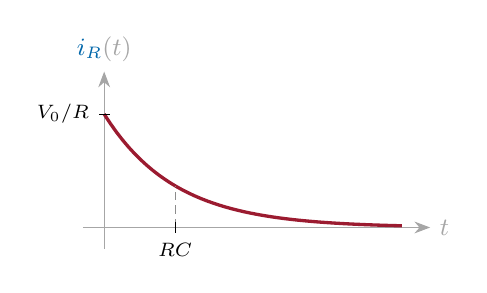
\begin{tikzpicture}[x=0.9cm,y=0.9cm]
  \tax{-0.3}{4.6}{-0.3}{2.2}{$t$}{$\iR(t)$}
  \draw[crv, domain=0:4.2, samples=50] plot (\x, {1.6*exp(-\x)});
  \yt{1.6}{$\Vo/R$}
  \draw[gdash] (1,0) -- (1,{1.6*exp(-1)}); \xt{1}{$RC$}
\end{tikzpicture}
\end{center}

\solstep{3}{Energy}
Energy delivered to the capacitor during $[0, t]$:
\[
  \Pcol{w_C(0, t)} = \tfrac12 C\vC(t)^2 - \tfrac12 C\Vo^2 = \tfrac12 C\Vo^2\big[e^{-2t/RC} - 1\big] < 0 .
\]
It is negative: the capacitor gives energy back. Energy dissipated in the resistor:
\[
  \Pcol{w_R(0, t)} = \int_0^t R\,\iR^2\,d\tau = \frac{\Vo^2}{R}\int_0^t e^{-2\tau/RC}\,d\tau
  = \tfrac12 C\Vo^2\big[1 - e^{-2t/RC}\big] .
\]
$w_C + w_R = 0$: all the energy taken from the capacitor is dissipated in the resistor. As
$t \to \infty$ the whole initial energy $\frac12 C\Vo^2$ ends up as heat.

\begin{examplebox}[Example 17.8 --- two capacitors and a switch]
\begin{minipage}[c]{0.44\linewidth}
\centering
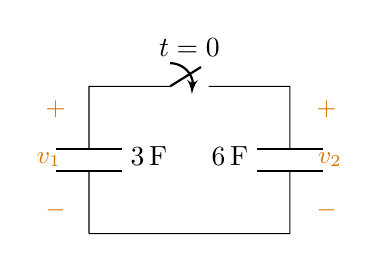
\begin{tikzpicture}[scale=0.85]\twoCap\end{tikzpicture}
\end{minipage}\hfill
\begin{minipage}[c]{0.52\linewidth}
$v_1(0^-) = 0$, $v_2(0^-) = 3\V$. The switch closes at $t = 0$. Find $v_1(0^+)$ and the stored
energy at $0^-$ and at $0^+$.
\end{minipage}
\end{examplebox}

\solution

\solstep{1}{Charge balance}
Take each current $i_k$ into the $+$ terminal of its capacitor. KCL gives $i_1 + i_2 = 0$: the
current leaving one capacitor enters the other. Integrating from $0^-$:
\[
  3\big(v_1 - 0\big) + 6\big(v_2 - 3\big) = 0 .
\]
For $t > 0$ the switch is closed, so KVL gives $v_1 = v_2$:
\[
  3v_1 + 6(v_1 - 3) = 0 \quad\Rightarrow\quad v_1(t) = v_2(t) = 2\V \quad (t > 0).
\]
Here the capacitor voltages \emph{do} jump: closing the switch forces two different voltages to
be equal, and an impulse of current flows from one capacitor to the other.

\solstep{2}{Energy}
\[
  \Pcol{E(0^-)} = \tfrac12 \cdot 3 \cdot 0^2 + \tfrac12 \cdot 6 \cdot 3^2 = 27\Jl,
  \qquad
  \Pcol{E(0^+)} = \tfrac12 (3 + 6) \cdot 2^2 = 18\Jl .
\]
$9\Jl$ is missing. Where did it go?

\solstep{3}{The missing energy}
Real switches and wires have some resistance $R$. Put a resistor $R$ in series with the switch.
The two capacitors in series act as $C_s = \frac{3 \cdot 6}{3 + 6} = 2\F$ with the initial
voltage difference $3\V$, so, as in Example 17.7, the current is $\frac{3}{R}e^{-t/2R}$ and the
energy dissipated in $R$ is
\[
  \Pcol{w_R} = \int_0^\infty R\,\Big(\frac{3}{R}\Big)^2 e^{-t/R}\,dt = \frac{9}{R}\cdot R = 9\Jl ,
\]
whatever $R$ is. The $9\Jl$ is dissipated in the resistance of the switch, however small it is.
With $R \to 0$ the current becomes an impulse, but the lost energy stays $9\Jl$.

%==============================================================
\section*{Summary}

\begin{center}
\small
\renewcommand{\arraystretch}{1.35}
\begin{tabular}{@{}>{\raggedright}p{3.6cm} >{\raggedright\arraybackslash}p{10.3cm}@{}}
\toprule
\textbf{Topic} & \textbf{Result}\\
\midrule
step, ramp, impulse & $\int_{-\infty}^t \delta = u$, $\int_{-\infty}^t u = r$; a jump of size $a$ at $t_0$ differentiates to $a\,\delta(t - t_0)$\\
sifting & $f(t)\,\delta(t - t_0) = f(t_0)\,\delta(t - t_0)$ for continuous $f$\\
capacitor & $i = C\,dv/dt$, \ $v(t) = v(t_0) + \frac1C\int_{t_0}^t i\,d\tau$; DC: open circuit\\
energy & $w = \frac12 C v^2 \geq 0$: stored, not dissipated\\
initial condition & charged $C$ $\equiv$ uncharged $C$ $+$ $\Vo u(t - t_0)$ in series $\equiv$ uncharged $C$ $\parallel$ $C\Vo\,\delta(t - t_0)$\\
connections & parallel $C_{eq} = \sum C_k$; series $1/C_{eq} = \sum 1/C_k$, initial voltages add\\
division & $i_1 = \frac{C_1}{C_1 + C_2}\,i_s$; \ $v_1 = \frac{C_2}{C_1 + C_2}\,v_s + \frac{C_1 V_{10} - C_2 V_{20}}{C_1 + C_2}$\\
$0^-$ to $0^+$ & bounded $i_C$ $\Rightarrow$ $v_C(0^+) = v_C(0^-)$; only an impulse of current makes $v_C$ jump\\
RC discharge & $v_C = \Vo e^{-t/RC}$; all stored energy dissipated in $R$\\
\bottomrule
\end{tabular}
\end{center}

\end{document}
